\section{Systems Under Test}
\label{sec:systems}

We compare four screening arms on the same prompt-only examples: TypeSafe Jev \citep{typesafe2026jevmodels,deusser2026jevbenchmark}, Cloudflare Clef and Clef-flash on Workers AI \citep{cloudflare2026clef,cloudflare2026clefflash}, and Amazon Bedrock Guardrails \citep{aws2024bedrockguardrails}. Every arm scores user text before any chat model runs. Stacks pair one typed decision model with the guardrail; they are evaluated in later sections but are not separate provider products.

\textbf{Typed decision models.}
Jev uses model id \texttt{jev-1.13.0} on the TypeSafe API. Requests follow the public Jev benchmarking harness: a fixed \emph{state} string (the prompt) and one or more typed questions (Noul yes/no probabilities, Choice labels, or Score rubrics) \citep{appliedml2026jevbenchmarking,deusser2026jevbenchmark}. Clef and Clef-flash use the same question shape on Cloudflare Workers AI with model handles \texttt{@cf/cloudflare/clef} and \texttt{@cf/cloudflare/clef-flash}. We pin weights revision \texttt{Cloudflare/clef} as in the study configuration. Hosted context limits differ (64{,}000 tokens for Clef versus 24{,}576 for Clef-flash); Workers AI may truncate a longer \texttt{state} and still return scores, and the scorer records truncation when it occurs.

\textbf{Bedrock Guardrails.}
The guardrail arm calls \texttt{ApplyGuardrail} in \textbf{detect-only} mode on \textbf{INPUT} text in AWS region \texttt{us-east-2}, using guardrail id \texttt{b4119czfeoh1} (version 1). We request content filters only: Hate, Insults, Sexual, Violence, Misconduct, and Prompt Attack. Denied topics, word lists, and grounding checks are disabled so latency and cost reflect the six filters alone. Each example triggers a single guardrail assessment with action \texttt{NONE}; we do not apply an automatic block at the API. Filter strengths (low, medium, high) and the block bit under each strength are derived offline from the saved assessment, using the documented rule that low blocks only \texttt{HIGH} bands, medium blocks \texttt{HIGH} and \texttt{MEDIUM}, and high also blocks \texttt{LOW} \citep{aws2024bedrockguardrails}. Headline stack metrics use medium strength unless noted otherwise.

\textbf{Category crosswalk.}
Dataset labels do not align one-to-one with Bedrock filter names. Before any test metric was computed, we published a per-dataset map from gold harm categories to filter subsets (for example, ToxicChat jailbreak to Prompt Attack, JailbreakBench harmful goals to Prompt Attack only in the pre-registered headline). OpenAI Moderation self-harm heads map to an empty filter set by design. GoEmotions and Emotion labels are affect classes, not Bedrock harm filters; for those sets the guardrail arm reports whether the comment would be blocked, not emotion accuracy.

\textbf{Stack policies without extra API calls.}
Union, intersection, and cascade policies are deterministic functions of stored decision-model probabilities and stored guardrail block bits. They never issue additional Jev, Clef, or Bedrock requests. Union blocks if either the guardrail blocks at the chosen strength or the model probability exceeds a tuned threshold $t$. Intersection blocks only when both fire. Cascade blocks when $P(\text{harm}) \ge t_{\mathrm{high}}$, allows when $P(\text{harm}) \le t_{\mathrm{low}}$, and otherwise defers to the guardrail block bit at medium strength. Thresholds $t$, $t_{\mathrm{high}}$, and $t_{\mathrm{low}}$ are fit on development rows only (see Section~\ref{sec:datasets}).

\begin{figure}[t]
  \centering
  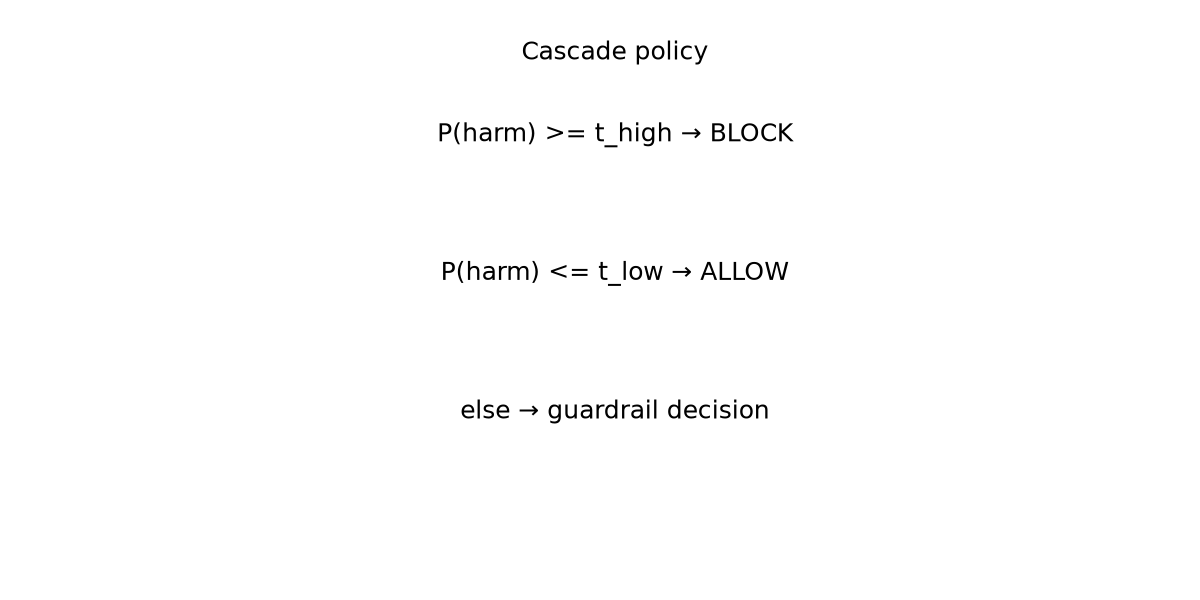
\includegraphics[width=0.72\linewidth]{../outputs/figures/20261020T040920Z_90c5fd13/cascade_flowchart.png}
  \caption{Cascade policy: a high model score blocks, a low score allows, and scores in the middle band defer to the guardrail block decision at medium strength.}
  \label{fig:cascade}
\end{figure}

\textbf{Protocol checks.}
Step~3 smoke tests passed for Jev, Clef, and Clef-flash; a second scoring pass hit the response cache. Guardrail scores feed the core-pack table after bands were recomputed from cached assessments with normalized filter names. A separate harness run reproduced published Jev intervals on six overlapping benchmarks before the full eleven-dataset pack was scored.
